\section {primer \& measurements}

In this section we will describe how rolling shutter mechanism works and then introduce our frequency-shift keying modulation and demodulation scheme based on the rolling shutter camera. In addition, we will state the unsynchronized issue of transmitter and receiver. 

\subsection{Rolling Shutter Channel Model}
\subsubsection{Rolling Shutter Operation}

\begin{figure}[!t] %move forward
	\centering
	\begin{subfigure}[h]{0.3\textwidth}
		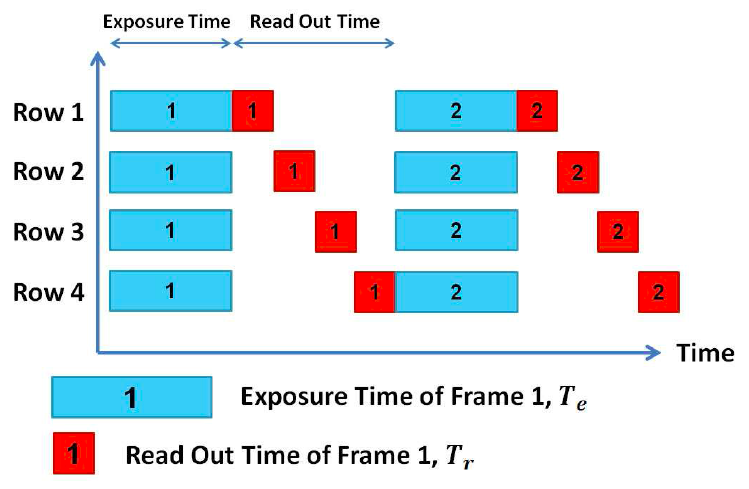
\includegraphics[width=\textwidth]{fig/global_shutter.png}
		\caption{Global Shutter Operation}
	\end{subfigure}
	~
	\begin{subfigure}[h]{0.15\textwidth}
		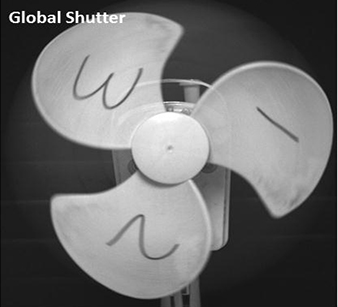
\includegraphics[width=\textwidth]{fig/fan_global}
		\caption{Global Shutter Example}
	\end{subfigure}
	\\
	\begin{subfigure}[h]{0.3\textwidth}
		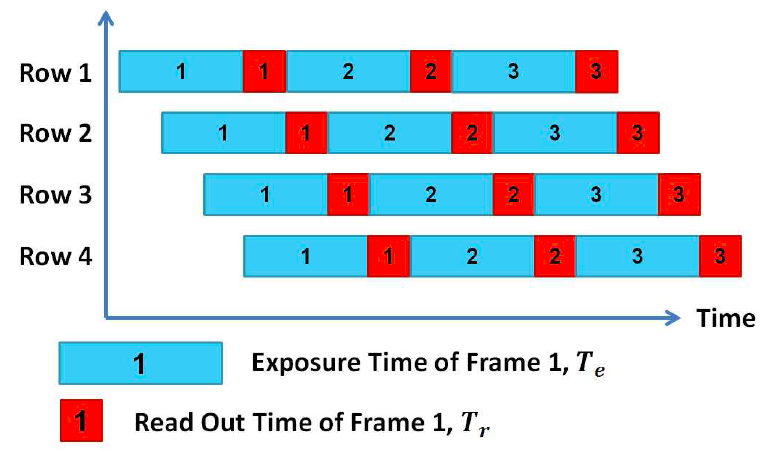
\includegraphics[width=\textwidth]{fig/rolling_shutter.png}
		\caption{Rolling Shutter Operation}
	\end{subfigure}
	~
	\begin{subfigure}[h]{0.15\textwidth}
		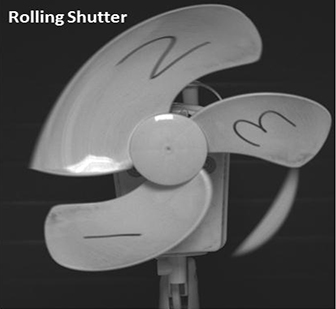
\includegraphics[width=\textwidth]{fig/fan_rolling}
		\caption{Rolling Shutter Example}
	\end{subfigure}
\caption{Shutter mechanisms}
\label{fig:compare_shutter}
\end{figure}

\autoref{fig:compare_shutter} compares global and rolling shutter operation \cite{imagesensor}. Global shutters, which are commonly implemented on CCD sensors, expose all pixels on the sensor simultaneously and gather incoming light over all pixels during the exposure time. 
Although some CMOS sensors use a global shutter, the majority found in the consumer market utilize a rolling shutter. 
One of the key properties of a rolling shutter camera sensor is its sequential read-out architecture. 
As in most CMOS sensors there is no per pixel storage to hold the accumulated charge during the exposure operation, the exposure period happens right before each read-out operation. 
The read-out architecture can process charge voltage signals one row at a time. 
Since the read-out durations of two rows cannot overlap, each of the exposure durations of a row of pixels is shifted by a fixed amount of read-out time (represented by $T_r$ in \autoref{fig:RollingShutter}), resulting in the so-called rolling shutter operation.
For each pixel, the incoming intensity modulated signal is integrated for a time period called exposure time (represented by $T_e$ in \autoref{fig:RollingShutter}). 

\begin{figure}[!t]
  \centering
  %\hspace{3em}
  % 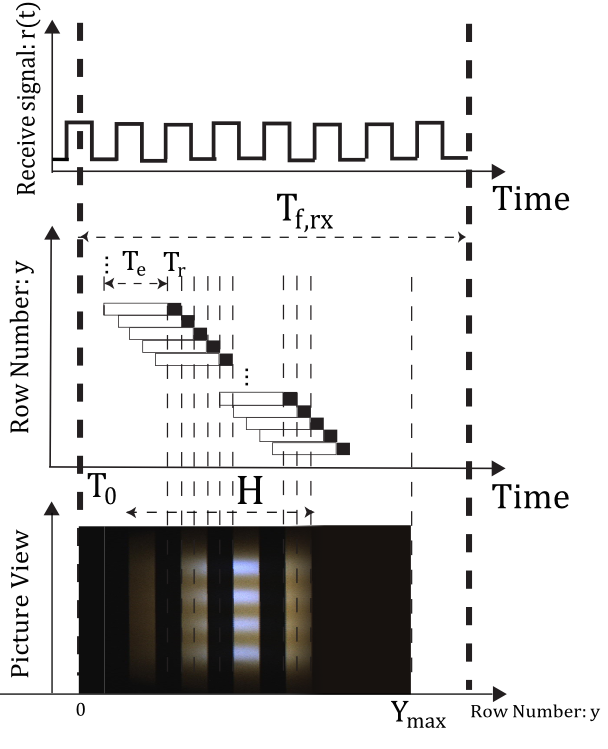
\includegraphics[scale=0.35]{fig/RollingShutter2}
  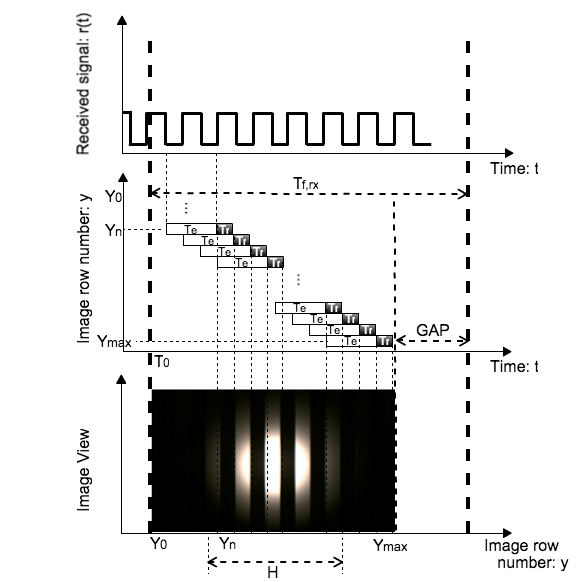
\includegraphics[scale=0.45]{pic/rollingshutter.png}
  \caption{The receiving operation of a rolling shutter camera sensor. Top: the original received signal; middle: the exposure and read-out processes; bottom: the resulted image. $T_{f,rx}$: receiving frame duration; $T_e$: exposure time; $T_r$: read-out time.}
  \label{fig:RollingShutter}
\end{figure}

\autoref{fig:RollingShutter} shows the receiving operation of a rolling shutter camera sensor to an intensity modulated signal.
Assume the original received signal in time is given by $r(t)$, which includes the signal from the transmitted light and other ambient interference. Considering the direct integration operation taking place during exposure and the rolling shutter operation, the intensity of a pixel in $y$-th row in the image, $I[y]$, which also represents the total amount of photons received by the pixel during exposure, is given by:

\begin{equation}
  I[y]=\int^{T_0+y T_r+T_e}_{T_0+y T_r} r(t) dt, \; 0 \leq y \leq Y_{\max},
  \label{eq:rollingshutter}
\end{equation}

where $T_r$ is the read-out time, $T_e$ is the exposure time, $T_0$ is a reference time point that corresponds to the start of the exposure time of the first row of pixels in the image, and $Y_{\max}$ is the number of rows of pixels in the image. Note that the transmitting light might not illuminate all rows in the image. In that case, the transmitted signal is only observed in $I[Y_{\operatorname{top}} \leq y \leq Y_{\operatorname{top}}+H]$, where $H$ represents the height of the image area illuminated by the transmitting light. 

The direct integration operation can be considered as a low-pass filter (or a moving average filter), and thus $I[y], 0 \leq y \leq Y_{\max}$ is a filtered version of the original received signal $r(t)$. The filter distorts high frequency components in the received signal, especially the ones with a frequency higher than $1/T_e$. 


\subsubsection{Time Gap in the Frame Duration}
Utilizing \autoref{eq:rollingshutter}, if the transmitting light occupies all rows of pixels in the image, the end of exposure of the last row in this image frame is $T_0 + Y_{\max} T_r + T_e$, while the start of exposure of the first row in the next image frame is $T_0 + T_{f,rx}$. The \textbf{time gap} between these two events is $T_{f,rx} - Y_{\max} T_r - T_e$, when $T_e$ is small, is significant for most cameras. 
This is the amount of time during which the camera is not performing any exposure operation, i.e., not receiving the transmitted signal. Signal transmitted during this time period is lost.  

\autoref{tab:readout} summarizes both the values of this time gap (without subtracting the exposure time $T_e$) and the percentage of time contributed by this time gap compared to a frame duration. Note that for some cameras, this could be up to half of the receiving frame duration. In addition, in the case that the transmitting light does not illuminate all rows in the image, this time gap could further increase. 

\subsubsection{Channel Characteristics}
In summary, the single-LED-to-rolling-shutter-camera channel exhibits two major characteristics:
\begin{enumerate}
  \item The signal that can be obtained from the image is a low-pass filtered version of the original received signal in time. The filter create distortions in high frequency components.
  \item The receiving process is not continuous. This can be considered as a form of channel fading; when it takes place, the channel loss is infinite. The ratio of signal lost is determined by a constant time gap that depends on camera parameters, and the size of the image area illuminated by the transmitting light. A smaller image area corresponds to a higher ratio of signal lost.
\end{enumerate}



\subsection{Rolling Shutter Frequency-Shift Keying \\(RS-FSK) Modulation }

The fundamental idea of RS-FSK is to use the square waves of a number of different \textbf{frequencies} as different symbols, mapped to different bit patterns of the same length. The signal of the $i$-th symbol is represented by the fundamental frequency $f_i$ of the square wave:
\begin{equation}
	s_i(t)= I_{\max} \left \lceil \frac{\cos (2 \pi f_i t)}{2} \right \rceil
\end{equation} where $I_{\max}$ is the maximum output intensity of the transmitting light. 

A frequency modulation is advantageous in the following aspects:
%\begin{itemize}
%\item
(1) The transmitted frequency can be demodulated by receivers with different sampling rate, as long as the sampling rate satisfies the Nyquist rate requirement. This implies that cameras with different read-out time are all compatible to a single transmission signal format.
(2) Demodulation is still possible when some segments of signal samples are lost in a symbol period, as long as the longest remaining signal segment has a length larger than the transmitted signal period. This addresses the time gap challenge previously described.
(3) The average intensity stays the same for all symbols, implying that the transmission is not observable by human eyes as long as the frequency is higher than 100 Hz. 
%\end{itemize}

In addition, a square wave has some key properties which make it suitable for our purposes:
%\begin{itemize}
(1) It survives the moving average filtering mechanism due to the exposure operation, as long as the signal period is not an integer multiple of the exposure time. This is true even for very long exposure time. Most important of all, the fundamental frequency of the square wave remains the same and accurately observable after filtering.
(2) It is extremely simple and can be implemented with cheap microcontrollers or PWM driver chips. No DAC is needed to output signal at different amplitude levels.
(3) The modulation supports dimming by transmitting a modified square wave at the same frequency, but with different ratio of ON state and OFF state, i.e., duty cycle. 

\autoref{fig:freq_strip} shows the received images of different transmitting frequencies.
%We will introduce the demodulation process in~\autoref{sec:demodulation}.
%\end{itemize}

\begin{table}[!t]
\hspace{-20em}
\small
\centering
\caption{Summary of Camera Parameters}
   \tabcolsep=0.05cm
    \begin{tabular}{|c|c|c|c|c|}
    \hline
                    % & Image Resolution & Frame Rate & Measured & Time Gap (ms)    \\
                    % &   ($X_{\max}$ x $Y_{\max}$)                &  (fps)          &  Read-out &  (Percentage of       \\ 
                    % &  &  & Time ($\mu$s) &  Frame Duration)   \\ 
      %& Image Resolution & Frame Rate & Measured Read-out & Time Gap (ms)    \\
      %&   ($X_{\max}$ x $Y_{\max}$)                &  (fps)          & Time ($\mu$s) &  (Percentage of       \\ 
      %&  &  &  &  Frame Duration)   \\  

    & Image           & Frame  & Measured    &  Time Gap (ms)    \\
    & Resolution                & Rate   & Read-out    &  (Percentage of   \\ 
    & ($X_{\max}$ x $Y_{\max}$) & (fps)  & Time ($\mu$s) &  Frame Duration)  \\  
    \hline \hline

    Point Grey Flea3 & 2048x1080          & 30         & 14.73             & 17.42 (52.27\%) \\ \hline

    Apple iPhone 6 Plus  & 1920x1080      & 30      & 21.42                   & 10.20 (30.60\%) \\ \hline

    Apple iPhone 5s  & 1920x1080          & 29.98      & 20.65                   & 11.03 (33.10\%) \\ \hline
    %Apple iPhone 4S  & 1920x1080          & 29.87      & 24.48                   & 7.04 (21.03\%) \\ \hline
    
    HTC New One      & 1920x1080          & 29.94         & 19.08              & 12.79 (38.30\%) \\ \hline
    Samsung Galaxy S4  & 1920x1080          & 29.93         & 25.53           & 5.84 (17.48\%) \\ \hline

    %Apple iPhone 4   & 1280x720           & 29.97      & 44.88                   & 1.05 (3.15\%)  \\ \hline
    %HTC Desire HD    & 800x480            & 29.08      & 55.18                   & 7.90 (22.97\%) \\ \hline
    %Google Nexus One & 720x480            & 30.57      & 59.66                   & 4.07 (12.45\%) \\ \hline
    \end{tabular}
    \label{tab:readout}
\end{table}


\subsection{Demodulation}
\label{sec:demodulation}
The transmitted signal period is the inverse of the transmitted signal frequency $f_i$. 
To obtain the \textbf{signal period}, we need to know the pixel width of strip in the received image first. 
%In \autoref{fig:rx_strip}, 
As rows of pixels are sequentially obtained with sampling period $T_r$, one cycle of square wave transmission results in a pair of bright strip and dark strip in the image. 
The sum of whole widths is given by
\begin{equation}
W= \frac{1}{f_i T_r} \qquad \textrm{.}
\label{eq:widthtofreq}
\end{equation}

% \begin{figure}[!t]
% 	\centering
% 	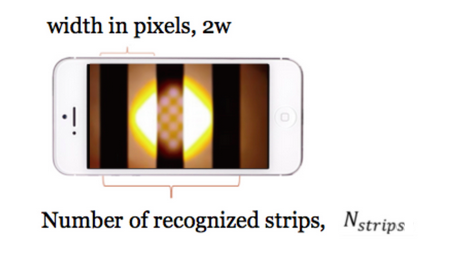
\includegraphics[scale=0.5]{fig/strip4.png}
% 	\caption{Received strips: w pixel}
% 	\label{fig:rx_strip}
% \end{figure}
\begin{figure}[!t]
\centering
  \begin{subfigure}[h]{0.12\textwidth}
  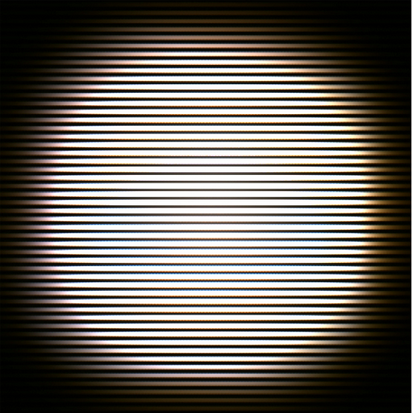
\includegraphics[width=\textwidth]{fig/strip1.png}
  \caption{8000 Hz}
  \end{subfigure}
  ~ 
  \begin{subfigure}[h]{0.12\textwidth}
  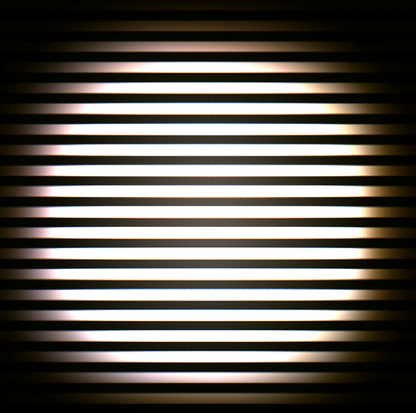
\includegraphics[width=\textwidth]{fig/strip2.png}
  \caption{4000 Hz}
  \end{subfigure}
  ~ 
  \begin{subfigure}[h]{0.12\textwidth}
  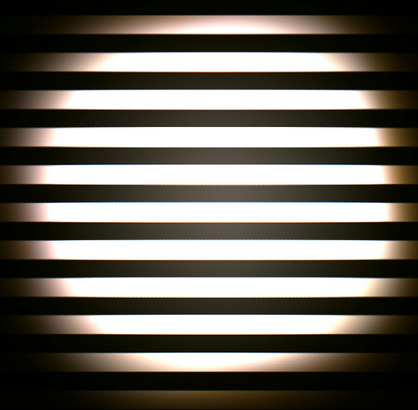
\includegraphics[width=\textwidth]{fig/strip3.png}
  \caption{2000 Hz}
  \end{subfigure}
\caption{Received images of different transmitting frequencies.}
\label{fig:freq_strip}
\end{figure}

Note that the width of the bright strip could be larger than the width of the dark strip in the image. This is due to blooming, the overflow of charge from a saturated pixel into its neighboring pixel~\cite{el2005cmos}. We thus consider the widths of the bright strip and the dark strip together in the calculation, to average out the effect. Since $W$ might not be an integer, averaging the observed widths over a large image area would help to improve the accuracy of the estimate of the width. Then, the transmitted period $1/f_i$ can be calculated with \autoref{eq:widthtofreq}. 

To have a more robust method to accurately determine the period of the signal, i.e., the average width of a pair of bright and dark strips in the image, we modified a well-known pitch detection algorithm (PDA), YIN~\cite{de2002yin}, that is originally designed to determine the fundamental frequency of a segment of audio signal in speech or music. We chose to use a method that operates in time domain, so that computationally expensive Fourier Transform operation can be avoided. 

We start by summing up all pixels in each row
\begin{equation}
	I[y]=\sum^{X_{\max}}_{x=1} I[x][y] \qquad \textrm{,}
\end{equation}
obtaining a one-dimensional signal, where $I[x][y]$ is the intensity (luminance)\footnote{If the obtained image is in RGB instead of grayscale, it needs to be converted to obtain the luminance information.} of the pixel at location $(x,y)$ in the received image. This operation uses pixels in different columns for redundancy, averaging out noises that exists in different columns of pixel. 

To find the period of the periodic signal presented in $I[y]$, a difference function may be constructed:
\begin{equation}
	d_\Delta(\delta)=\sum^{H/2-1}_{y=1} (I[y] - I[y+\delta])^2
\end{equation}
and we search for the values of $\delta$ that are closest to zero. Note that $\delta$ represents both the shift in space in number of pixels and the shift in time in multiples of read-out time of the camera. As pointed out in~\cite{de2002yin}, using the difference function instead of the standard autocorrelation function (ACF) can avoid a large portion of the error caused by change of amplitudes in the signal, causing by the change of luminance in different rows of pixels. An added advantage is that subtraction is computationally more efficient than multiplication. 

Another possible source of error happens at small $\delta$ values, since when $\delta<\frac{1}{f T_r}$, the difference function could produce a large value due to the fact that we use square waves - there is no significant change of signal amplitude except at the sharp transitions. We instead use cumulative mean normalized difference function (CMNDF)~\cite{de2002yin} to mitigate this problem:
\begin{equation}
	d_\Delta'(\delta) =\begin{cases} 1, & \textrm{if\;} \delta=\{0,1\} \\
	d_\Delta(\delta) / \left [ (1/\delta) \sum^\delta_{j=1} d_\Delta(j) \right ] & \textrm{otherwise.} \end{cases}
\end{equation}

The function now starts from $1$ at $\delta=0$ and remains large with small $\delta$ values, and only drops below $1$ when $d_\Delta'(\delta)$ falls below average. The smallest local minimum in $d_\Delta'(0 \leq \delta \leq H/2-1)$ is then located and serves as the period estimate of the received signal.  

Using CMNDF, the system can determine the period of the transmitted signal with a resolution of read-out time. However, as the period of the signal is not always an integer multiple of the read-out time, i.e., the sampling period, the output could results in error up to half of the read-out time. We again resort to the method proposed in~\cite{de2002yin} - to use parabolic interpolation to estimate the location of the actual minimum that could exist between samples. Assuming that $\hat{\delta}$ is the integer value that corresponds to the smallest minimum in $d_\Delta'(\delta)$, this method only needs three function values, $y_{-1}=d_\Delta'(\hat{\delta}-1)$, $y_{0}=d_\Delta'(\hat{\delta})$, and $y_{+1}=d_\Delta'(\hat{\delta}+1)$, to determine the new estimate:
\begin{equation}
	\hat{\delta}'=\hat{\delta}+\frac{y_{+1}-y_{-1}}{2 (2 y_0 - y_{+1} - y_{-1})}
\end{equation}

With parabolic interpolation, our modified YIN algorithm can very accurately determine the period of the transmitted signal. Note that the output of the algorithm is in pixel. It can be converted back to be in unit of time by multiplying the number with $T_r$.


\subsection{Unsynchronized Transmitter and Receiver}

\begin{figure*}[!t]
   \centering
   \begin{subfigure}[h]{0.25\textwidth}
      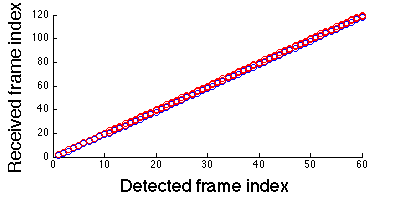
\includegraphics[width=\textwidth]{fig/tx_15_new.png}
      \caption{tx = 15 fps} \label{fig:tx_15fps}
   \end{subfigure}%
   ~
   \begin{subfigure}[h]{0.25\textwidth}
      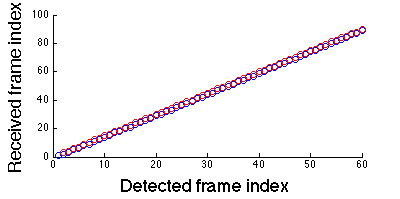
\includegraphics[width=\textwidth]{fig/tx_20_new.png}
      \caption{tx = 20 fps} \label{fig:tx_20fps}
   \end{subfigure}%
   ~  
   \begin{subfigure}[h]{0.25\textwidth}
      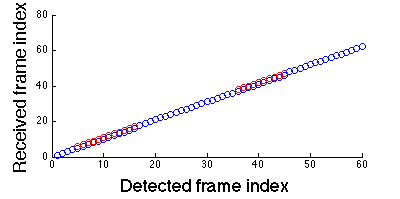
\includegraphics[width=\textwidth]{fig/tx_29_new.png}
      \caption{tx = 29 fps} \label{fig:tx_29fps}
   \end{subfigure}%
   ~
   \begin{subfigure}[h]{0.25\textwidth}
      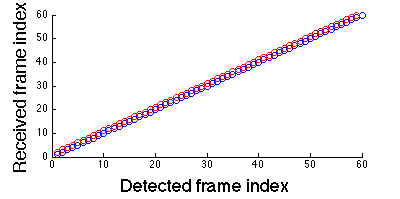
\includegraphics[width=\textwidth]{fig/tx_30_2_new.png}
      \caption{tx = 30 fps} \label{fig:tx_30fps_2}
   \end{subfigure}%
   \\
   \begin{subfigure}[h]{0.25\textwidth}
      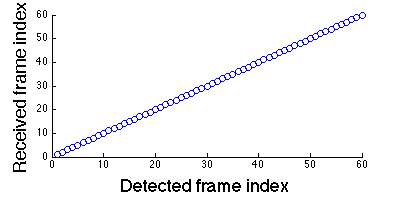
\includegraphics[width=\textwidth]{fig/tx_30.png}
      \caption{tx = 30 fps} \label{fig:tx_30fps}
   \end{subfigure}%
   ~   
   \begin{subfigure}[h]{0.25\textwidth}
      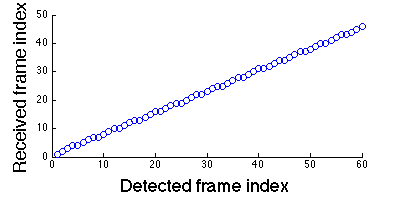
\includegraphics[width=\textwidth]{fig/tx_40.png}
      \caption{tx = 40 fps} \label{fig:tx_40fps}
   \end{subfigure}%
   ~
   \begin{subfigure}[h]{0.25\textwidth}
      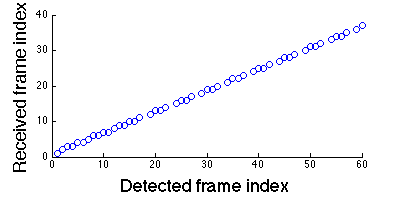
\includegraphics[width=\textwidth]{fig/tx_50.png}
      \caption{tx = 50 fps} \label{fig:tx_50fps}
   \end{subfigure}%
   ~
   \begin{subfigure}[h]{0.25\textwidth}
      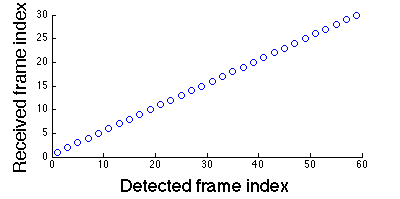
\includegraphics[width=\textwidth]{fig/tx_60.png}
      \caption{tx = 60 fps} \label{fig:tx_60fps}
   \end{subfigure}%
   \caption{Received frame patterns under different tx fps}
   \label{fig:diff_tx}
\end{figure*}

\subsubsection{The Problem}

As the transmitting light and the receiving camera are not synchronized, the transmitting frame rate and the receiving frame rate are usually not the same. 
As mentioned is~\cite{hu2013lightsync}, the received frame rate exhibits more variability for several reasons. It described as follows: HTC One X camera appears to record videos are 24 fps, but the camera callback API can only support saving the frames at 15 to 20 fps. The callback slows down when there is insufficient memory available in the system. The frame rate on the Samsung Galaxy S III is only stable if the CPU is locked to its maximum frequency with its setCPU app. Otherwise, it fluctuates hugely between 21 to 29 fps for an entirely white foreground, and have an average of around 25 fps. Even when the frame rate appears steady, the inter-frame interval still varies. 

% In our design, we assume that the ratio $fps_{tx}$ / $fps_{rx}$ is not more than 2 or less than 0.9, which means the receive frame rate is between 15 and 33 fps when the transmitting frame rate is 30 fps. Note that this can be changed with straightforward modifications to our design to allow a larger variability of frame rate. 

\textbf{Received frame patterns.} We follow the experiement in~\cite{hu2013lightsync}, given various potential combinations of the transmitting and receiving frame rates, we perform a simple experiment to study the received frame pattern. We transmit the data at several frame rates, and record the video with the PointGrey Flea3 camera~\cite{pointgrey_flea} with 30 fps. 

\autoref{fig:diff_tx} shows the received frame pattern. For each received frame, we can detect which of the originally transmitted frames corresponds to it, and plot a circle for each detected frame. When two or more detected frame indices correspond to the same received frame index, this captured frame contains a \textbf{mixture of two or more transmitted symbols}. When two or more received frame indices correspond to the same detected frame index, these captured frames have \textbf{redundant transmitted symbols}. Any gap between consecutive received frame indices indicates a \textbf{symbol loss}. 

At 15 fps and 20 fps, we capture at least one complete frame with a full symbol. However, other frames show that the mixed frames and redundant frames are also possible due to random phase offsets. When the transmitting rate is close to the receiving rate - 30 fps, mixed frames would be received for a few consecutive frames. Even when the transmitting frame rate is exactly 30 fps, mixed frames can still occur, in which case, it would always be the case received due to the constant phase offset, as shown in \autoref{fig:tx_30fps_2}. In the other case, a single transmitted symbol would always be received in each frame, as shown in \autoref{fig:tx_30fps}.
As the transmitting rate increases further, we start to experience mixed and missed symbols at times.

% Since the camera records the videos at 30 fps, detecting the same number of transmitted frames requires receiving far more frames at a low transmitting rate. Therefore, the scales of the vertical axis are different across the subfigures of \autoref{fig:diff_tx}.

\subsubsection{The Probability}
\label{sec:unsync}
To figure out the symbol loss and mixed frame problems, we first want to know how often do they happen, thus we derive the probabilities under different conditions. In addition, we want to know what factors affect them and how to address them. 

\textbf{Case I: When the transmitting frame rate is higher than the receiving frame rate,}
there could be symbol loss, defined as no part of the transmitting frame duration of a particular symbol is covered by the exposure time of any receiving image frame. 
\autoref{fig:miss} illustrates the missing symbols. 
Let the transmitting frame duration be $T_{f,tx}$ (symbol time), the receiving frame duration be $T_{f,rx}$, and the Y size of the image area illuminated by the transmitting light be $H$. The gray part is the time gap that the camera is not receiving the transmitting symbols. If $T_{f,tx} < T_{f,rx} - H T_r$, which means the transmitting symbols may appear in the gray part, then a symbol loss is possible. In that case, the probability of a symbol lost is given by
\begin{equation}
	P_{\operatorname{miss}}=\frac{T_{f,rx} - H T_r - T_{f,tx} }{T_{f,rx}} \qquad \textrm{.}
\end{equation}

We can see that the probability of the symbol loss in \autoref{fig:miss} is around 1/2, which means there is a symbol loss followed by every received symbol. 


A more common event which could happen when the transmitting frame duration and the receiving frame duration are different is that in a single image frame there could be multiple image areas each corresponding to a symbol. In other words, a mix of different symbols in a single receiving image frame. 
\autoref{fig:mix} illustrates the mixed frames. If the boundary between two consecutive transmitting symbols locates in the red part, during which the camera is receiving the transmitting symbols, then there is a mixed frame.
The probability for this event is given by
\begin{equation}
P_{\operatorname{mix}}=\begin{cases} \frac{H T_r}{T_{f,tx}}, & \textrm{if\;} T_{f,tx} \geq H T_r \\
1, & \textrm{otherwise.} \end{cases}
\end{equation}

We can see that the probability of the mixed frame in \autoref{fig:mix} is around 1/3. 

\begin{figure}[!t]
  \centering
  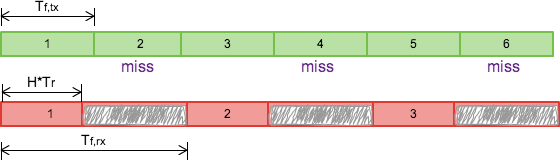
\includegraphics[scale=0.35]{fig/miss.png}
  \caption{Missing symbol illustration.}
  \label{fig:miss}
\end{figure}

\begin{figure}[!t]
  \centering
  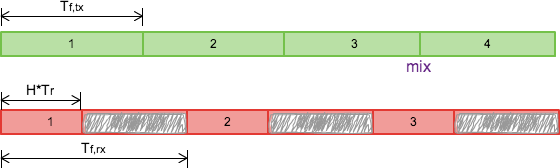
\includegraphics[scale=0.35]{fig/mix.png}
  \caption{Mixed frame illustration.}
  \label{fig:mix}
\end{figure}

A mixed frame is a very common and periodic event. Even when the transmitting and the receiving frame durations are very close to each other, mixed frames would be received for a few consecutive frames. After receiving a few frames with only a single symbol, consecutive mixed frame would appear again. \autoref{fig:mix_photo} shows the received frame with mixed symbols.
If the boundary of the image areas corresponding to different symbols is not determined, then the period detection algorithm would output one value. The value would usually be closer to the signal period of the symbol that occupies a larger image area, but usually has a large error.  

% \begin{figure}[!t]
%   \centering
%   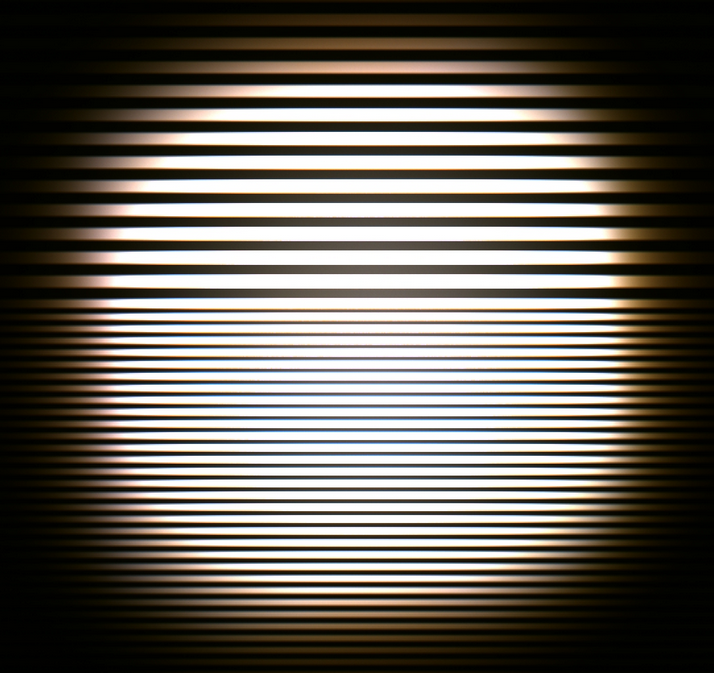
\includegraphics[scale=0.1]{fig/mix_photo.png}
%   \caption{Received frame with mixed symbols.}
%   \label{fig:mix_photo}
% \end{figure}

\textbf{Case II: When the transmitting frame rate is lower than the receiving frame rate,}
a redundant symbol is possible. Although no information is lost, the receiver still needs to detect a redundant symbol so that it can be dropped to obtained the correct symbol sequence.  


On the other hand, a mixed frame is also possible in this case. The probability for a mixed frame is given by
\begin{equation}
P_{\operatorname{mix}}=\frac{H T_r}{T_{f,tx}} \qquad \textrm{.}
\end{equation}
which is same as the probability in Case I.
We can see that the probability of the mixed frame in \autoref{fig:mix2} is around 1/3. 

According to the probability of lost symbol and mixed frame, the transmitting frame duration ($T_{f,tx}$), the receiving frame duration ($T_{f,rx}$), the height of the LED in the image ($H$), and the read-out time of camera sensor ($T_r$) and the factors which may affect the probabilities. We will introduce and evaluate how well our design address these issues in the following chapters.


\begin{figure}[!t]
\centering
  \begin{subfigure}[h]{0.12\textwidth}
  
\includegraphics[width=\textwidth]{pic/5c.JPG}
  \caption{iPhone 5c}
  \end{subfigure}
  ~ 
  \begin{subfigure}[h]{0.12\textwidth}
  
\includegraphics[width=\textwidth]{pic/5s.JPG}
  \caption{iPhone 5s}
  \end{subfigure}
  ~ 
  \begin{subfigure}[h]{0.12\textwidth}
  
\includegraphics[width=\textwidth]{pic/6plus.JPG}
  \caption{iPhone 6Plus}
  \end{subfigure}
\caption{Received images of different devices with same transmitting frequency}
\label{fig:freq_strip_iphones}
\end{figure}
